\section{Reputation Systems}
\label{sec:reputation_systems}

On the internet, we interact with a lot of strangers. People can be anonymous. It is common to see individuals identify themselves only with a nick names \cite{Resnick2000}. In these circumstances, it is hard to build trust with each other. Online trade on the internet can be compared to the market of lemons as described in \cite{Akerlof1970}. A mechanism is required that incentivises individuals to act with honest intention. Internet scale systems use \textit{Reputation Systems} to foster trust between the users. A Reputation System collects, distributes and aggregates feedback about participants' past behaviours. Reputation systems require at least three properties \cite{Resnick2000}:

\begin{enumerate}
  \item Long-lived entities that inspire an expectation of future interaction;
  \item Capture and distribution of feedback about current interactions (such information must be visible in the future); and
  \item Use of feedback to guide trust decisions.
\end{enumerate}

Through reputation system, these properties can be applied to a) Users and b) Entities

\subsection{Reputation System for users}

Reputation system for users helps other individuals know what quality items to expect from a given user. Online systems like eBay, Amazon and other platforms that allow two sided transactions employ these techniques. On eBay, after a transaction is done, a buyer can leave either a positive, neutral or negative feedback for a seller. The feedback amounts to +1, 0 or -1 feedback points. A seller over a period of time accumulates feedback points from various buyers which becomes her feedback profile. A new buyer can use the feedback profile to decide if the seller is reliable enough.

\begin{figure}[!htb]
  \centering
  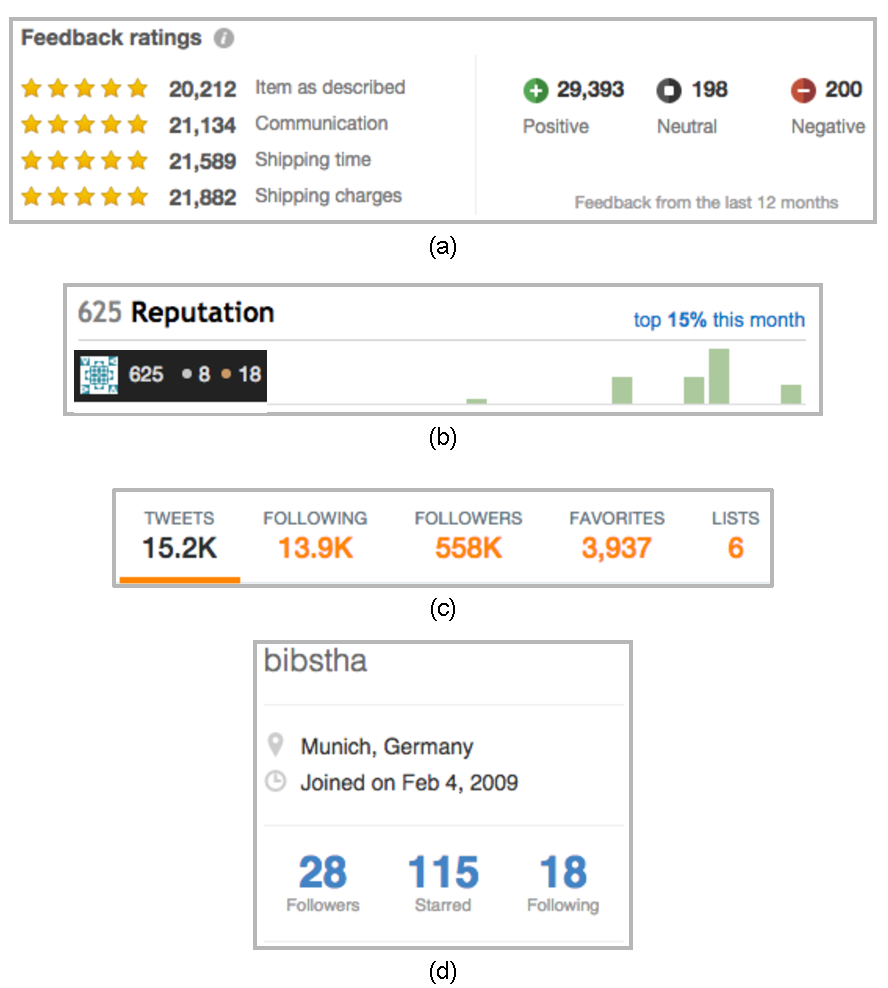
\includegraphics[width=11cm]{figures/rs_for_users.pdf} 
  \caption{Different reputation systems for users: (a) eBay feedback ratings, (b) StackOverflow User reputation, (c) Twitter reputation and (d) Github user follow information}
  \label{fig:rs_for_users}
\end{figure}

Reputation system for users also span beyond auction and e-commerce systems. QnA site  StackOverflow.com rates users by letting others choose the most helpful answers to a question. Users are encouraged to answer in the most comprehensive and helpful manner. This leads to higher quality answers. Product review sites (such as www.epinions.com) offer rating services for product reviewers (the better the review, the more points the reviewer receives).

Sites with \textit{follow} feature allow users to subscribe to the activities of other users. These systems build a directed graph structure. Each node is a user. Incoming vertices show people following the user while outgoing vertices show who she is following. Reputation is considered higher if she has high number of followers. In twitter.com, higher reputation means more people listen or like the users' posts. In github.com, higher reputation means more people are interested in the users' code contributions.

Reputation system for users portray a characteristic of a user. Political scientist Robert Axelrod calls this the ``Shadow of the future'' \cite{Axelrod1984}. An expectation that people will consider one another's pasts in future interactions constrains behaviour in the present.

\subsection{Reputation Systems for entities}

When trading on the Internet, it is not possible to directly interact with the items of trade. It is hard to determine the quality of products when there are multiple vendors selling products that are similar in visuals and written specifications. Reputation Systems for entities add visual measures as quality attributes. They gathers opinion from previous consumers to form a qualitative opinion of the entities and help new consumers form opinions.

\begin{figure}[!htb]
  \centering
  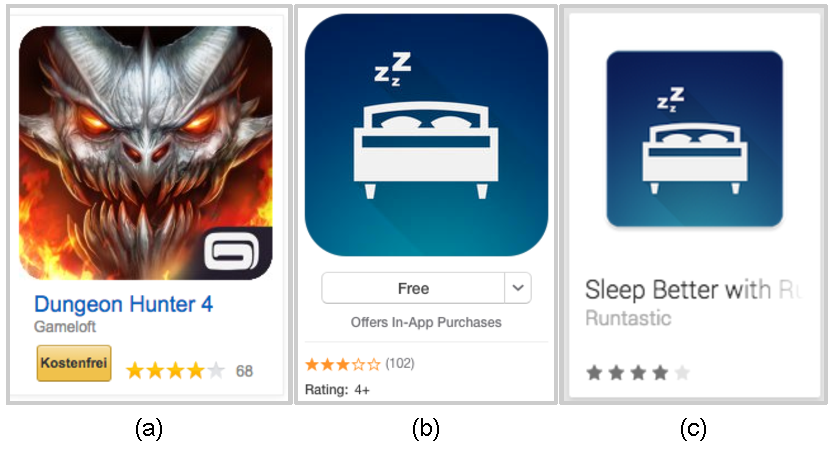
\includegraphics[width=12cm]{figures/rs_for_entities.pdf} 
  \caption{Different reputation systems for entities: (a) Amazon Appstore ratings, (b) Apple's Appstore ratings and (c) Google's PlayStore ratings}
  \label{fig:rs_for_entities}
\end{figure}

Reputation system for entities are used widely online. Amazon allows rating a product on a scale from 1 to 5 (1 very bad, 5 very good). Products of lower rating are assumed to be of lower quality and therefore make lower sales.

Apple's App Store and Google's Play Store only support reputation systems for entities. Both use the same model: users can rate an application in the scale of 1 to 5 stars (more stars means higher quality). App stores display the aggregate average. Apple's App store features categorization of ratings and reviews based on \emph{application versions}. This allows users to get more accurate review of the application based on current status. A developer can fix or update their applications based on user feedbacks. The Play Store shows aggregate rating of an application regardless of the version.

On Github.com, reputation of a project depends upon multiple factors. Being an OpenSource platform, the importance of a project can be determined by the number of \textit{stars} by other users. Community interest can be determined by the number of \textit{contributors} and number of \textit{watches} for the project. The \textit{last commit time} and \textit{number of commits} show the activity in the project. 

Github.com also makes communication between developers transparent and visible to everyone else. This inferred developer commitment, improved quality, increased the sense of community and created personal relevance which influences reputation management \cite{dabbish2012social}.

\subsection*{In context of S2Store}

S2Store can use the benefits of both reputation systems for users and entities.

\emph{Reputation system for users} can be used so a developer can follow the activities of another developer. Badges system can be used to add gamification elements to encourage developer contributions.

\emph{Reputation system for entities} are a must \cite{farmer2010building}\cite{Resnick2000}. They form the basic mechanisms for users to provide feedbacks to the developers about the quality of the software services.

\subsection{Reputation System Building Blocks}

A Reputation System is analyzed by breaking it down into the following building blocks \cite{Resnick2000}:

\begin{enumerate}
  \item The claim,
  \item Processes that compute the reputation,
  \item Routers that notifies other processes (sending messages to users, notify other dependent system processes, etc) after a reputation is calculated.
\end{enumerate}

\subsubsection{Claim}

A claim is an assertion of quality that a \textit{source} makes about a \textit{target}. Claims can be \textit{explicit} (a direct statement of quality by the source, e.g. ranking of apps by users) or \textit{implicit} (derived from other actions of the source towards the target, e.g. computing popularity by number of downloads of an app). Claims can also be a) qualitative type or b) quantitive type. Qualitative claims attempt to describe the quality of a reputable object, e.g. ``this is an exceptional restaurant'' or ``this app has beautiful color combination''. They could be expressed by text or pictorial reviews. Quantitative claims are measurable. They are easier to implement computationally and conceptually. Quantitave claims can be collected as \textit{Normalized Values} (expressed within the range of 0.0 to 1.0), \textit{Rank Values} (a rank is a unique positive number given to a set of items, e.g. an order of top 100 apps based on page views) or \textit{Scalar Values} (a number assigned to the reputable item as a grade, usually between upper and lower limits, e.g. rating movies in the imdb between 1 and 10).

\subsubsection{Processes that compute the reputation}

The claim collected goes through different processes that transform it into other formats. Processes can be counters, accumulators, averages, mixers,  ratios, etc. A \textit{Counter} increases by 1 everytime there is a claim, e.g. hit counters. \textit{Accumulator} sums up the scalar value given by sources to calculate the grand total. \textit{Averages} calculate the current running average including the new input. \textit{Mixer} combines two or more inputs into a single score according to a weighing formula. For \textit{Ratio}, the total number of inputs (the total) is counted. Then, the number of times the value is 1.0 (maximum between 0.0 and 1.0) is counted. With the two, a ratio is infered with a claim value of ``(hits) out of (total).''

\subsubsection{Routers}

When the reputation value is newly calculated or changed from existing value, different actions can occur. Update in reputation pass through \textit{an evaluator} that performs an ``If ... Then ...'' statement. Update can \textit{split} and notify multiple parts of the bigger system. Or it can \textit{combine} with other updates to form a combined reputation value.

The inputs, processing and routing can either happen in order (synchronous). Or it can send a signal to another process and terminate (asynchronous). The process to receive the signal can be reputation calculating process or one that belongs to the external application.

\subsection{Common Reputational Models}

These different building blocks can be combined in different ways. The common patterns in which they are combined are explained in this section.

\subsubsection{Favorites and Flags}

The ``Favorites and Flags'' model can be used to identify items that users find either exceptionally good (favorites) or exceptionally bad (flags). This model detects the outliers. Every time a user favorites or flags an item, its reputation either increases or decreases respectively.

Favorites and Flags can be used in three variants: a) vote to promote, e.g. Reddit, Digg, b) favorites for future reference or to show interest, e.g. starring projects in Github or Google Code, following users in Github c) Flag as abuse. This model is usually implemented using a \emph{counter} process.

\begin{figure}[!htb]
  \centering
  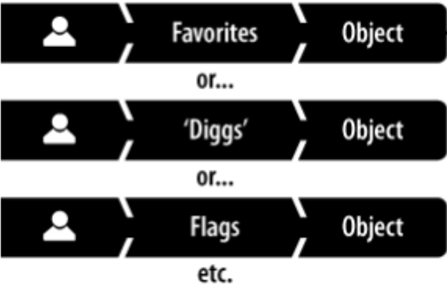
\includegraphics[width=5cm]{figures/rs_model_fav_and_flags.pdf} 
  \caption{Favorites, flags or send-to-friend models. (Source~\cite{farmer2010building})}
  \label{fig:rs_model_fav_and_flags}
\end{figure}

% TODO: Insert an image here

\subsubsection{Ratings}

Ratings model are used to get an explicit opinion about a reputable item. The upper and lower limit of the scale may vary from one variant to another. E.g. Internet Movie DataBase has a rating scale of 1 to 10, Google Play Store has a rating scale of 1 to 5. Ratings are gathered from multiple individual users and rolled up as a community average score for that target.

\begin{figure}[!htb]
  \centering
  
\includegraphics[width=5cm]{figures/rs_model_ratings.pdf} 
  \caption{Ratings model to rate individual objects. (Source~\cite{farmer2010building})}
  \label{fig:rs_model_ratings}
\end{figure}

\subsubsection{Reviews}

A review is a collection of ratings on different facets for a repuatble item. It also contains a text based freeform opinion.

\begin{figure}[!htb]
  \centering
  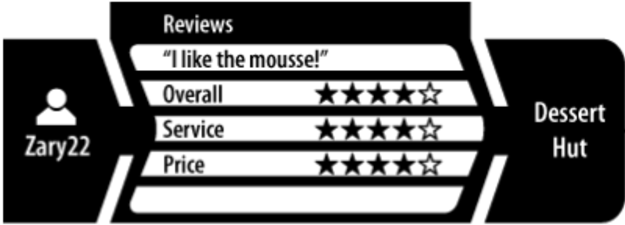
\includegraphics[width=6cm]{figures/rs_model_reviews.pdf} 
  \caption{Ratings include a text freeform opinion combined with other reputation models. (Source~\cite{farmer2010building})}
  \label{fig:rs_model_reviews}
\end{figure}

\subsubsection{Points}

Points are awarded to users based on their activity on the platform. If points are awarded properly, it encourages people to engage more on the platform, e.g. Stackoverflow awards users with points and badges for correctly answering questions. Please enage more for reputation.

\begin{figure}[!htb]
  \centering
  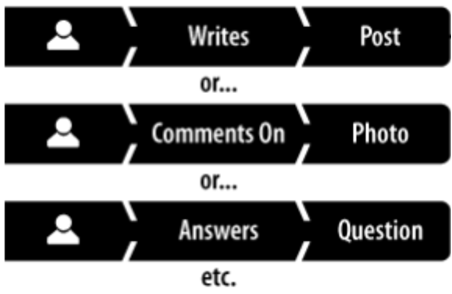
\includegraphics[width=5cm]{figures/rs_model_points.pdf} 
  \caption{Points are similar to favorites and flags but depends upon indirect action. (Source~\cite{farmer2010building})}
  \label{fig:rs_model_points}
\end{figure}

\subsection*{In context of S2Store}

\emph{Favorite and Flags} can be used as following:
\begin{enumerate}
  \item User can \emph{favorite or flag} an existing service.
  \item Developer can follow another developer.
  \item Developer can mark a context model as favorite, adding to its reputation.
\end{enumerate}

\emph{Ratings} can be combined with \emph{Reviews} to allow collection of qualitative feedback where users can express their satisfaction or frown with meaningful explanations.

\emph{Points} can be used in following ways:

\begin{enumerate}
  \item A point can be added to the service for each download. Uninstall would do the opposite.
  \item A point can be added to the context model for every service that associates itself with the context model.
\end{enumerate}

\subsection{Implicit Rating}
\label{subsec:implicit_rating}

In explicit rating, users explicitly tell the system what they think about something. Explicit rating gives accurate observation about an item. But explicit rating requires users to interrupt their normal browsing behavior \cite{claypool2001inferring}. Implicit rating uses less intruding methods. In general for e.g., users tend to read more articles than they rate. Users are also likely to review applications only if they find them very good or very bad \cite{Podkopajev2012}. Implicit rating evaluates the reputation through certain interest indicators based on user behaviors.

Girardello and Michahelles developed an app for Android called \emph{AppAware} as part of a voluntary research experiment \cite{girardello2010explicit}. The app collects events triggered every time a user installs, updates or removes any other app in their cell phones. These events are then shared with a central remote server. AppAware calculates the reputation of each app based on an assumption that good applications are not removed once installed, applications not liked are usually removed from the device. AppAware introduces an acceptance rate (reputation score) $v$ for an application $app$ as the value going from 0 to 100 computed with the formula in eq \ref{eq:appaware_a}, where $U$ is the set of users having at least one event for $app$ \cite{girardello2010explicit}.

\begin{equation}\label{eq:appaware_a}
  v(app)=\frac{\sum_{user \in U} last(app, user)}{|U|}
\end{equation}

\begin{equation}\label{eq:appaware_b}
  last(app,user) = \begin{cases}
    0 & \text{if last event for user for app = removed} \\
    90 & \text{if last event for user for app = installed} \\
    100 & \text{if last event for user for app = updated}
  \end{cases}
\end{equation}

According to eq \ref{eq:appaware_b}, the acceptance rate is based on the most recent event. \emph{Update} event is given more weight than \emph{install} because the assumption is that the user finds value in the app and keep it installed. \emph{Remove} event sets the acceptance rate to 0.

\subsection*{In context of S2Store}

The AppAware experiment from \cite{girardello2010explicit} shows good corelation between explicit rankings taken from Google's PlayStore and the collected implicit rankings. Therefore, eq \ref{eq:appaware_a} and \ref{eq:appaware_b} can be also used in S2Store. S2Store can track with the permission of user, when a new service is installed, uninstalled or updated and infer an implicit rating that can be combined with explicit rating to generate an aggregate reputation for services.